\section{The horizon decides what is learned; the optimizer decides where the residue goes}
\label{sec:behaviour}

A higher score is not by itself better therapy, so we read the transcripts as well as the
instruments. The cleanest statistic is deliberately the crudest: a \textbf{judge-free lexical
over-praise marker} --- a keyword pattern matched against the transcript with no model in the
loop, hence identical under any grader --- giving the share of therapist turns containing at
least one unearned-affirmation marker. It is kept as a direction check on the oracle-coded rates,
not as a measurement in its own right; the argument rests on the \emph{agreement} between the two.

\textbf{Turn-level reward teaches flattery in both optimizers.} From base rates of
$0.000$--$0.003$, the marker share at iteration 10 reaches $\mathbf{0.671}$ in \GRPO-$\Kz$ and
$\mathbf{0.210}$ in \PTO-$\Kz$ --- two turns in three, and one turn in five, containing unearned
praise. The oracle-coded over-praise rate on the same conversations tells the same story ($0.698$
and $0.299$), and the coded rate is significantly higher under $\Kz$ than $\Kf$ in the last 5--7
iterations for both optimizers under both graders (Figure~\ref{fig:overpraise}). The mechanism is
legible: Q1/Q2 ask a simulated patient how satisfied they felt, praising the patient raises
exactly that in the turn where it happens, and the cost lands turns later --- outside a $\Kz$
judge's window, inside a $\Kf$ judge's.

\textbf{Trajectory-level reward suppresses the drift in both.} The same marker reads $0.064$
(\GRPO-$\Kf$) and $0.045$ (\PTO-$\Kf$) at the endpoint --- roughly one turn in sixteen to
twenty-two, against base rates near zero. On the training oracle's coding, \GRPO-$\Kf$'s total
MI-inconsistency is flat over the whole run ($0.209 \rightarrow 0.210$) and \PTO-$\Kf$'s nearly
so ($0.177 \rightarrow 0.264$); the held-out judge reads both $\Kf$ arms as rising --- \GRPO\
$0.326 \rightarrow 0.628$, \PTO\ $0.370 \rightarrow 0.581$ --- but at well under half their
$\Kz$ siblings' endpoint rates ($1.050$ and $0.825$). The defensible sentence, and the one this
paper uses, is that the longer horizon \emph{slows the drift to a fraction of its turn-level
rate and removes its dominant channel}, in both optimizers --- not that it eliminates it.

\begin{figure*}[t]
\centering
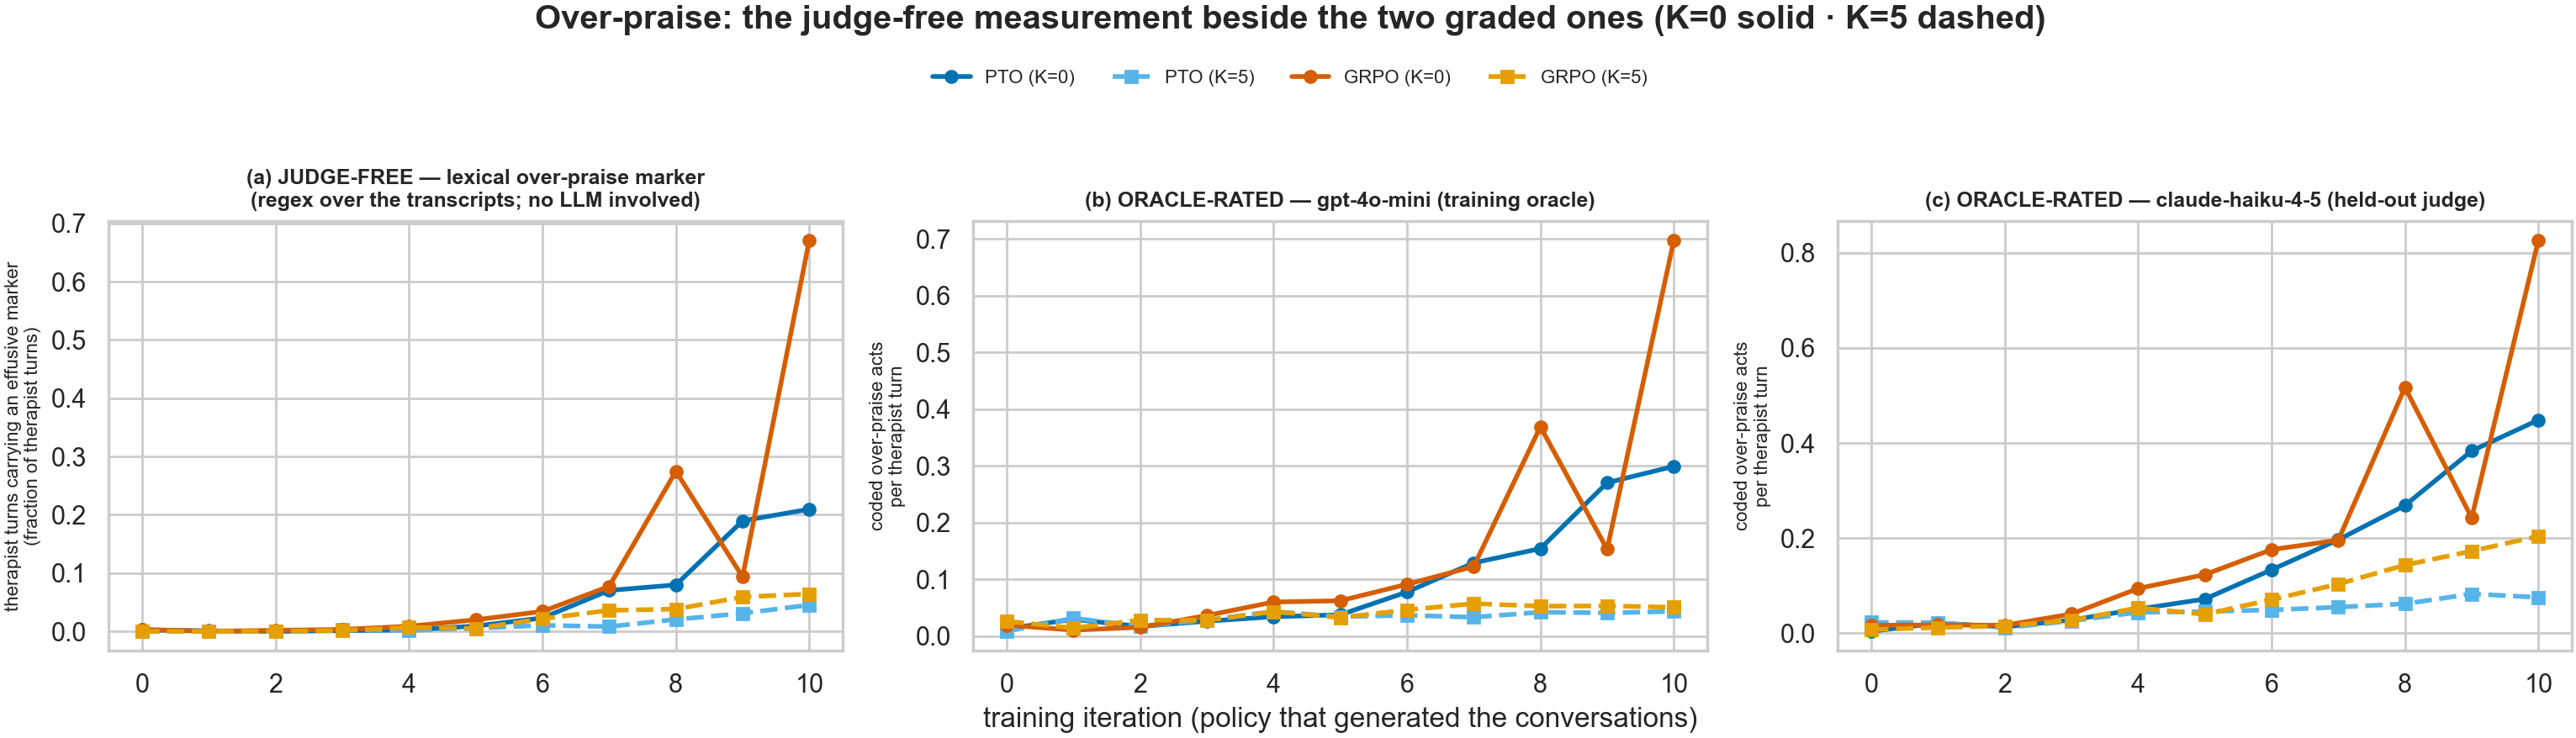
\includegraphics[width=0.98\textwidth]{figures/overpraise_judgefree.png}
\caption{Over-praise by iteration, all four arms, three ways: the judge-free lexical marker
(left; no model in the loop), and the oracle-coded rate under each grader (middle, right;
independent $y$-axes). Both $\Kz$ arms climb; both $\Kf$ arms hold near base. The judge-free
panel tells the same story as the rated ones, which is the point: the behavioural claim does not
rest on an LLM's judgement of an LLM.}
\label{fig:overpraise}
\end{figure*}

\textbf{Where the optimizers part ways is the residue.} In \PTO, suppressing over-praise is
accompanied by a \emph{relocation}: under the held-out coder, advice-without-permission is
significantly \emph{higher} in the $\Kf$ arm than the $\Kz$ arm in 6 of the last 7 iterations
(per-session counts) --- the inconsistency partially migrates to a channel whose cost the
five-turn window still does not expose. \GRPO\ shows only traces of the same migration (3
iterations), and instead substitutes a behaviour MI training wants more of: the $\Kf$ policy asks
significantly more questions per therapist turn at 7 of 10 iterations (mean \dz\,$0.64$;
deterministic text statistic), while \PTO's question rate does not move with $K$ at all. A
group-relative update that trains on all eight scored siblings appears to find the
ask-rather-than-affirm substitution that a best-vs-worst pair update does not --- we offer that
as the natural reading, not as a demonstrated mechanism (per-channel forests for both optimizers
in Appendix~\ref{app:tables}).
